\documentclass{article}

% Packages
\usepackage{graphicx} % required for inserting images
\usepackage{geometry}
\usepackage{amssymb}
\usepackage{amsmath}
\usepackage{comment}
\usepackage{mathtools, nccmath}
\usepackage{hyperref}

\newgeometry{vmargin={15mm}, hmargin={20mm}}
\title{EECS 199 - Pump and PH Testing System (Hardware and Software)}
\author{Ivan Tran (UID: 46403682)}

\begin{document}
    \maketitle

    \tableofcontents
    \newpage
    \section{Overview}
        \begin{flushleft}
            This report will detail the systems that we used to conduct the pump and pH testing experiments.
            \begin{itemize}
                \item \textbf{Pump Testing}: For the pump experiment, we tested the rate that volume was dispensed to see if it matches the product specification.
                \item \textbf{pH Testing}: For the pH experiment, we calibrated the pH module to see if it measured pH accurately. We then tested how the pH probe reading would change as we added acid and base solutions.
            \end{itemize}
        \end{flushleft}

    \section{Hardware Components Used}
    \begin{flushleft}
        \begin{itemize}
            \item 2x 12V Relays (\href{https://www.amazon.com/dp/B00LW15D1M/}{Product Page})
            \item 1x 12V Power Supply Adapter (\href{https://www.amazon.com/dp/B01GEA8PQA/}{Product Page})
            \item 2x Peristaltic Pumps (\href{https://www.amazon.com/dp/B07GWJ78FN/}{Product Page})
            \item 1x Atlas Scientific pH Probe and Sensor Module \href{https://www.amazon.com/dp/B00798612C/}{Product Page}
        \end{itemize}
    \end{flushleft}

    \section{Hardware}
        \subsection{Pump and pH Sensor Circuit Schematic}
            \begin{flushleft}
                A schematic for the pump and pH sensor circuit is shown in the image below. The pumps are connected to the GPIO pins 20 and 21. The SCL and SDA pins of the pH sensor are connected to the 
                \begin{figure}[!hbt]
                    \centering
                    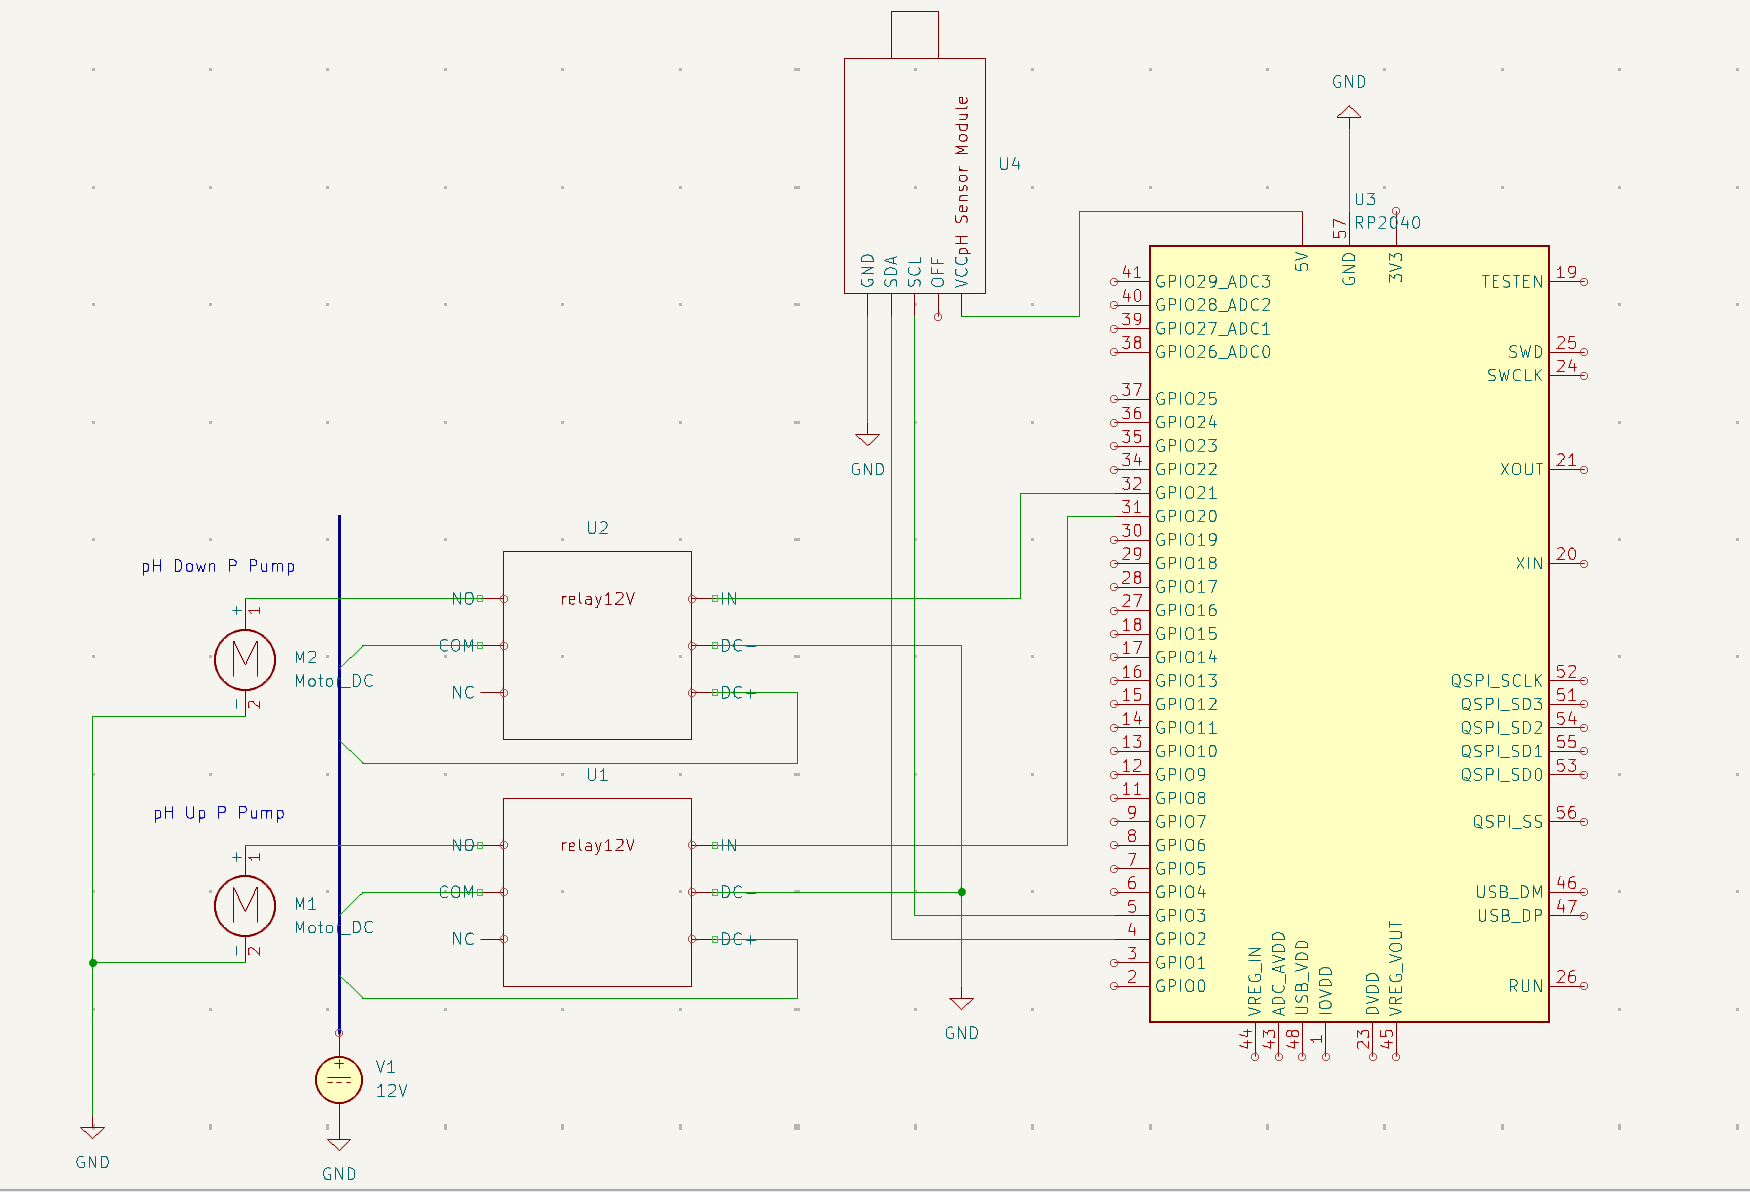
\includegraphics[width=0.50\linewidth]{assets/pumpAndPHTestingCircuitSchematic.png} % paste image w/i these brackets
                \end{figure}
            \end{flushleft}
        \subsection{Pump and pH Sensor Physical Circuit}
            \begin{flushleft}
                The physical circuit for the schematic is shown below.
                \begin{figure}[!hbt]
                    \centering
                    \includegraphics[width=0.50\linewidth]{assets/pumpAndPHTestingCircuitPhysical.png} % paste image w/i these brackets
                \end{figure}
            \end{flushleft}
        \newpage
    \section{Software}
        \subsection{Pump}
            \begin{flushleft}
                Our pumps are powered by an external 12V power supply. The code responsible for controlling the pumps is actually controlling the relays which determine whether the 12V power supply is powering the pumps are not. See the file $\text{pPumpCode.py}$ for more details.
            \end{flushleft}
        \subsection{pH Sensor}
            \begin{flushleft}
                Currently, we are using a python program to poll the data, but we have not integrated this program with the pumps yet. What we plan to do in Spring 2024 is to automate the pH of the solution that the pH sensor is measuring the pH of by having the pumps turn on based on the measured pH value of the solution.
            \end{flushleft}
    \section{3D Modeling}
        \begin{flushleft}
            We used one 3D model in the current iteration of the project which is a mount for the pumps. Below is an image showing the mount.
            \begin{figure}[!hbt]
                \centering
                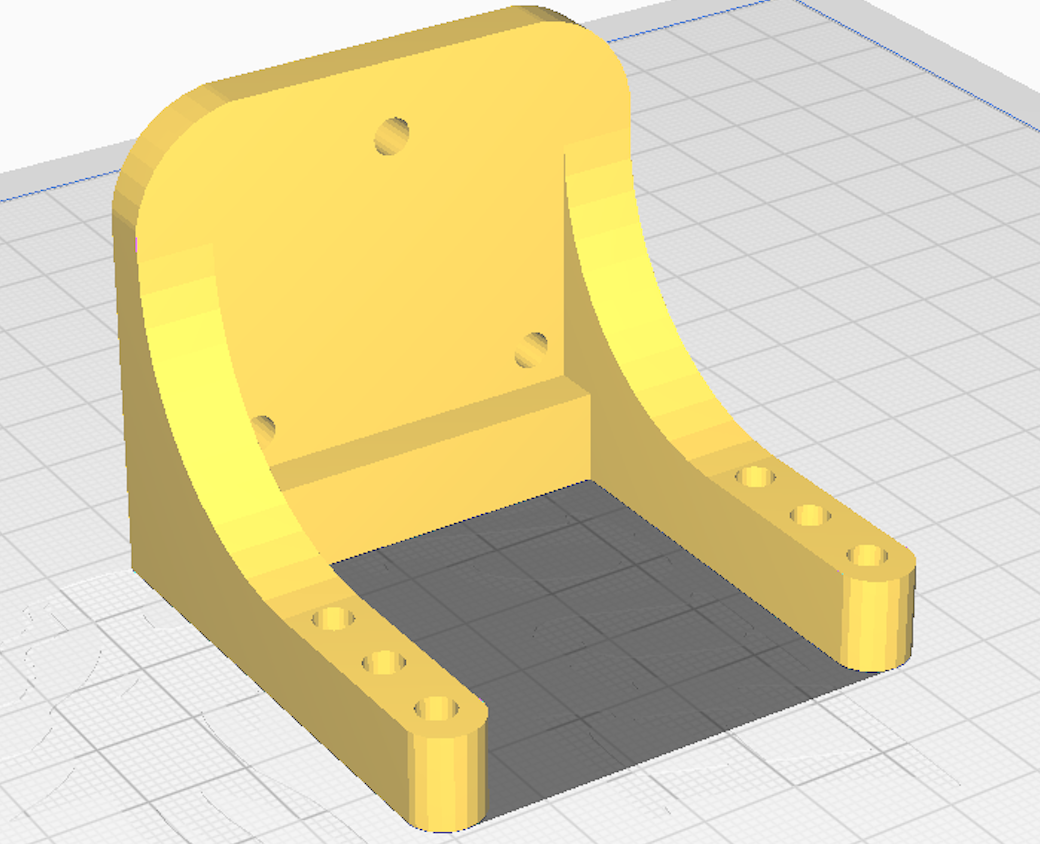
\includegraphics[width=0.50\linewidth]{assets/pPumpIsoView.png} % paste image w/i these brackets
            \end{figure}
        \end{flushleft}
        \begin{flushleft}
            This is what the mount looks like once the pump is mounted onto it and the mount is attached to a piece of plywood (2 mounts were used for 2 pumps)
            \begin{figure}[!hbt]
                \centering
                \includegraphics[width=0.35\linewidth]{assets/pumpMountedOnBoard.png} % paste image w/i these brackets
            \end{figure}
        \end{flushleft}
        \begin{flushleft}
            This is a temporary structure that we are using for the pumps (for testing and experimental purposes). Once we integrate the pumps into the hydroponics system, we will have a more suitable structure.
        \end{flushleft}
    \section{Resources}
        \begin{flushleft}
            Below shows a list of resources used to set up the hardware and software correctly:
            \begin{itemize}
                \item EZO pH Integrated Circuit: \href{https://files.atlas-scientific.com/pH_EZO_Datasheet.pdf}{link}
            \end{itemize}
        \end{flushleft}
\end{document}